\chapter{Solución propuesta}

En el presente capítulo se presenta la propuesta de diseño de la solución para el problema de investigación abordado en el presente trabajo, así como su implementación.
% Habiendo conocido las características que mejor describen a los atributos del presente trabajo, se puede decir que la base del método propuesto se puede desarrollar.

\section{Diseño de la solución propuesta} \label{Diseño de la solución propuesta}
En diseño de la solución propuesta se plantean las herramientas utilizadas y los pasos seguidos para la solución propuestas.

Las herramientas utilizadas en la presente investigación se muestran en el cuadro \ref{tab:Herramientas utilizadas}.

\begin{table}[H]
	{\centering
		\caption{Herramientas utilizadas.}
		\begin{tabular}{|c|c|c|}
			\hline 
			Herramienta & Versión & URL\\
			\hline
			\texttt{Python} & 3.8.8 & \url{https://www.python.org/}\\
			\hline
			\texttt{Imageio} & 2.9.0 & \url{https://imageio.readthedocs.io/}\\
			\hline
			\texttt{Latextable} & 0.2.1 & \url{https://pypi.org/project/latextable/}\\
			\hline
			\texttt{Matplotlib} & 3.3.4 & \url{https://matplotlib.org/}\\
			\hline
			\texttt{NumPy} & 1.20.1 & \url{http://www.numpy.org/}\\
			\hline
			\texttt{Pandas} & 1.2.4 & \url{https://pandas.pydata.org/}\\
			\hline
			\texttt{Seaborn} & 0.11.1 & \url{https://seaborn.pydata.org/}\\
			\hline
			\texttt{Scikit-learn} & 0.24.1 & \url{https://scikit-learn.org/}\\
			\hline
			\texttt{SciPy} & 1.6.2 & \url{https://docs.scipy.org/}\\
			\hline
			\texttt{Statsmodels} & 0.12.2 & \url{https://www.statsmodels.org/}\\
			\hline
			\texttt{Texttable} & 1.6.4 & \url{https://pypi.org/project/texttable/}\\
			\hline
		\end{tabular}
		
	\label{tab:Herramientas utilizadas}
	}
\end{table}

\subsection{Recolección de datos}
La primera fase es la recolección de datos. El objetivo es tener un archivo que contenga datos de los niveles de uno o más contaminantes del aire en años recientes y también del mismo lugar tener datos del número de egresos hospitalarios durante esos años.

\subsection{Selección y agrupación de datos}
Después de la recolección de datos se procede a seleccionar que datos van a ser utilizados para los experimentos. Para ello se utiliza \texttt{Python} con la librería \texttt{Pandas} \ref{tab:Herramientas utilizadas} que permite la manipulación de datos. 
Para la selección y agrupación de datos se sigue el procedimiento mostrado en la figura \ref{alg:a1}.

\begin{algorithm}
\caption{Selección y agrupamiento de datos}\label{alg:a1}
\begin{algorithmic}[1]
\State $a \leftarrow $ años de los que se obtuvieron datos
\For {$i \in a$}
    \State $contaminantes \leftarrow $ nombre del archivo .csv que contiene los datos de los contaminantes en el año $i$
    \State Leer en $contaminantes$ las columnas fecha y contaminante 
    \State $egresos \leftarrow $ nombre del archivo .csv que contiene los datos de los contaminantes en el año $i$
    \State Leer en $contaminantes$ las columnas fecha, padecimiento y estado
    \State $estado \leftarrow $ estado del que se quieren obtener datos
    \State Seleccionar en $contaminantes$ los datos del $estado$
\EndFor
\end{algorithmic} 
\end{algorithm}

\subsection{Visualización de la evolución de las variables}
Al ya tener seleccionados los datos a utilizar se procede a elaborar gráficos en \texttt{Python} \ref{tab:Herramientas utilizadas} que muestran la evolución de las variables en el tiempo. Para ello se generan los tipos de gráficos discutidos a continuación.

\subsubsection{Series de tiempo}
Se realizan series de tiempo en Python con ayuda de la librería  \texttt{Matplotlib}, \texttt{Scikit-learn} y \texttt{Seaborn} \ref{tab:Herramientas utilizadas}, ya que son herramientas accesibles que ayudan a la generación de este tipo de gráficos. %; en la figura \ref{serie_de_tiempo} se muestra un ejemplo de las series de tiempo generadas.

%\begin{figure}[h!]
%\setcounter{figure}{0} % por culpa de sciposter
%\captionsetup{type=figure} % por culpa de sciposter
%\begin{center}
%   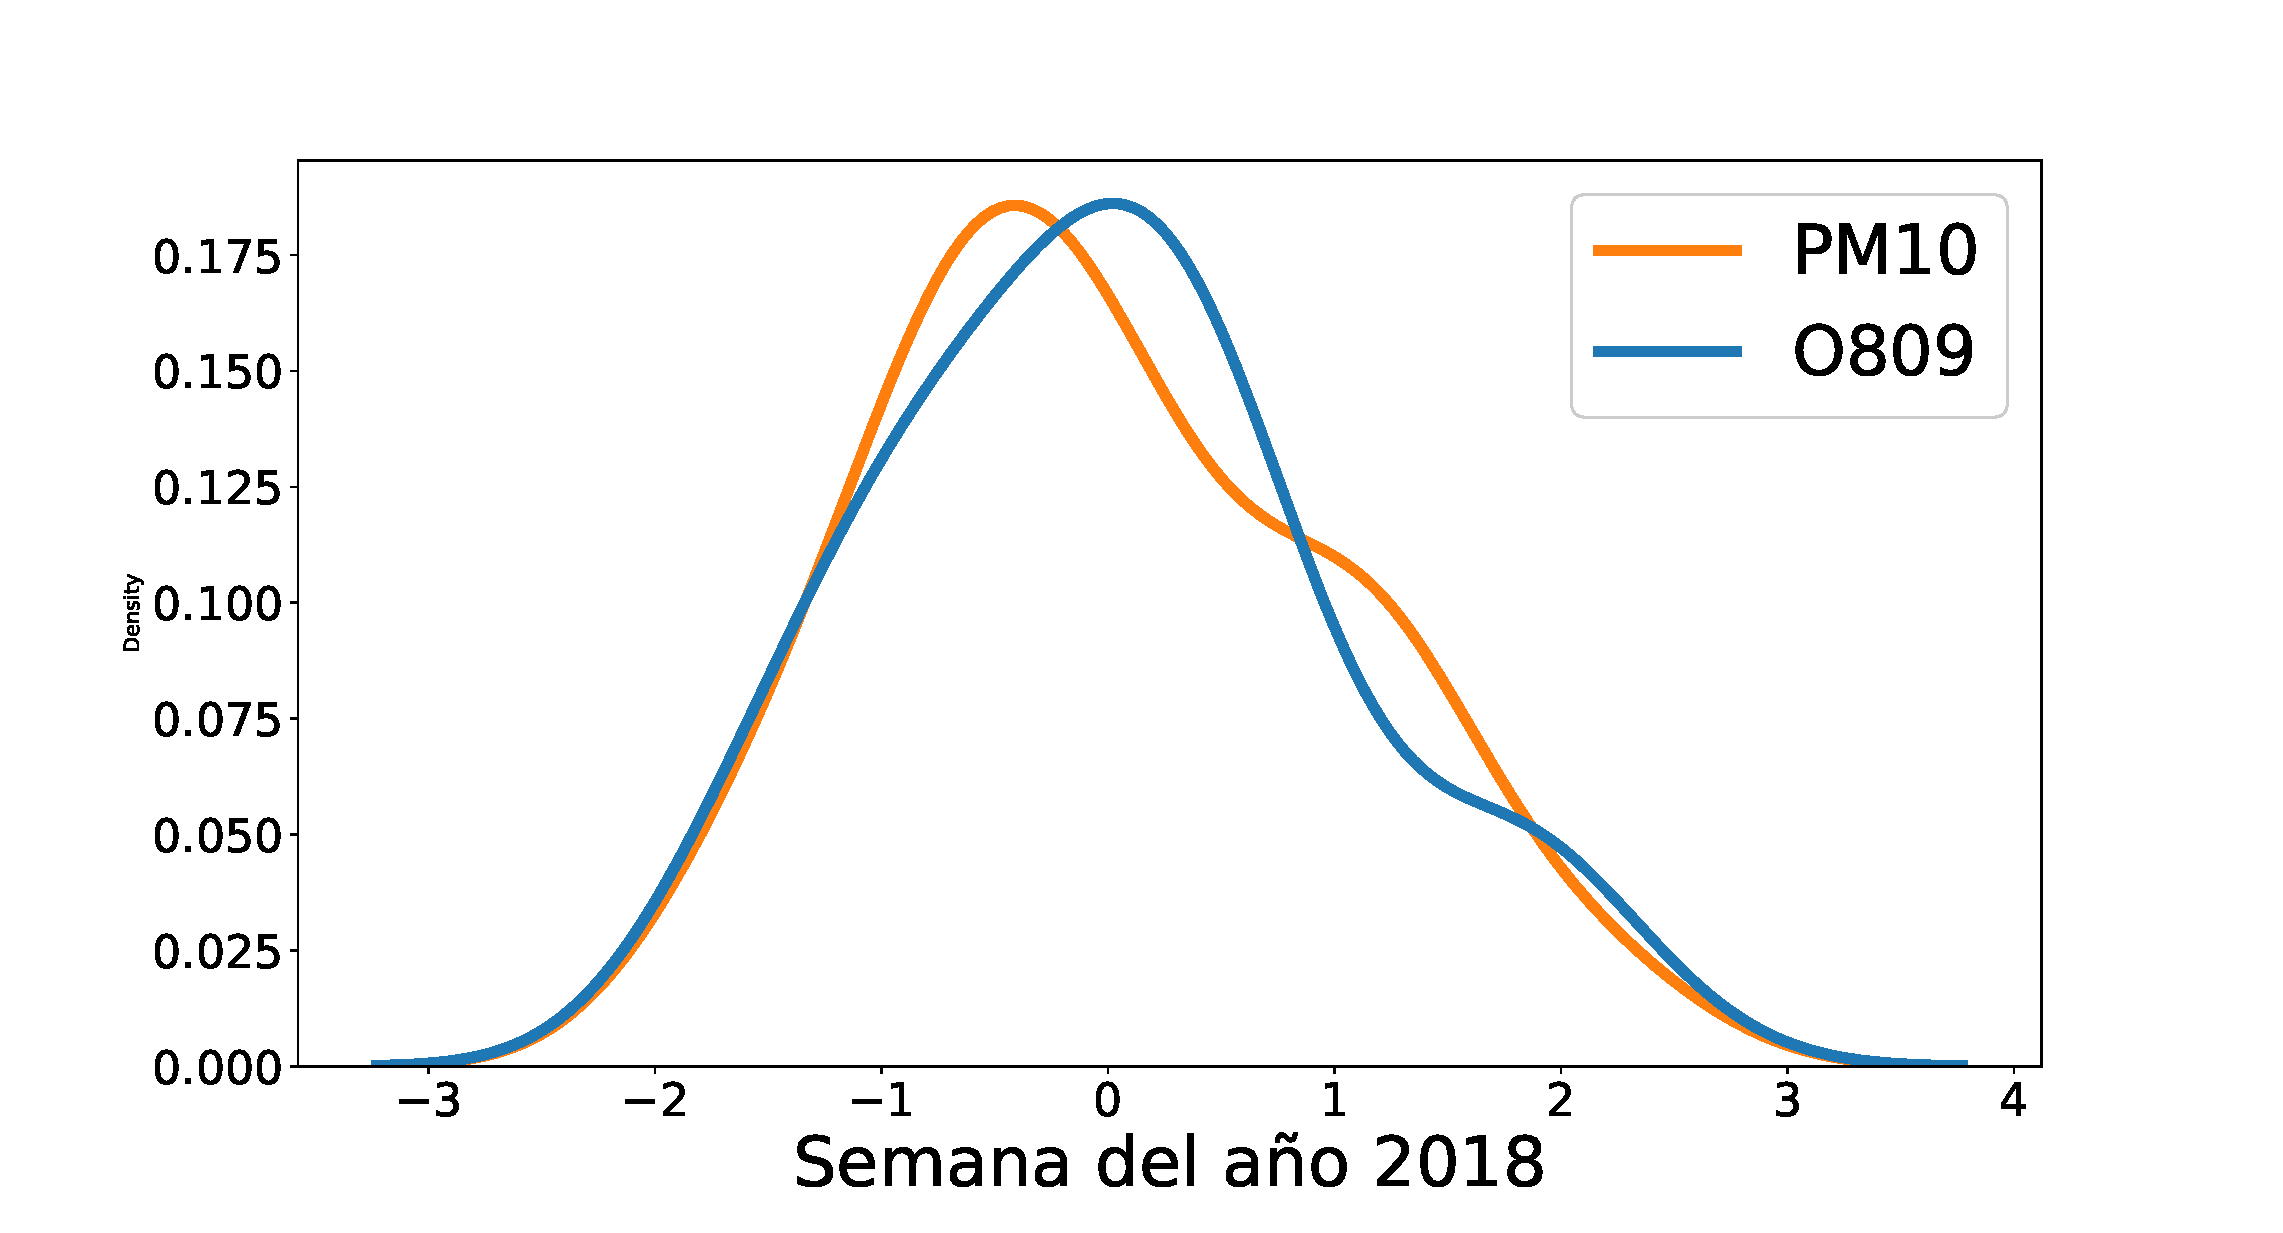
\includegraphics[width=1\textwidth]{PM10_O809_2018.eps}
%   \end{center}
%    \caption[Ejemplo de series de tiempo]{Evolución de los niveles de PM10 y el número de egresos diagnosticados con la CIE O809 en el 2018.}
%    \label{serie_de_tiempo}
%\end{figure}

\subsubsection{Gráficos de radar}
Los gráficos de radar o diagramas de telaraña son otra manera de visualizar un conjunto de datos. Sirven para comparar variables visualizando si existen valores o patrones de evolución en el tiempo similares entre ellas. Es por ello que en el presente trabajo se elaboran gráficos de radar con ayuda de \texttt{Python} y las librerías \texttt{NumPy} y \texttt{Matplotlib} \ref{tab:Herramientas utilizadas}. En la figura \ref{grafico_de_telaraña} se muestra un ejemplo de los gráficos de telaraña generados.

\begin{figure}[h!]
\setcounter{figure}{1} % por culpa de sciposter
\captionsetup{type=figure} % por culpa de sciposter
\begin{center}
   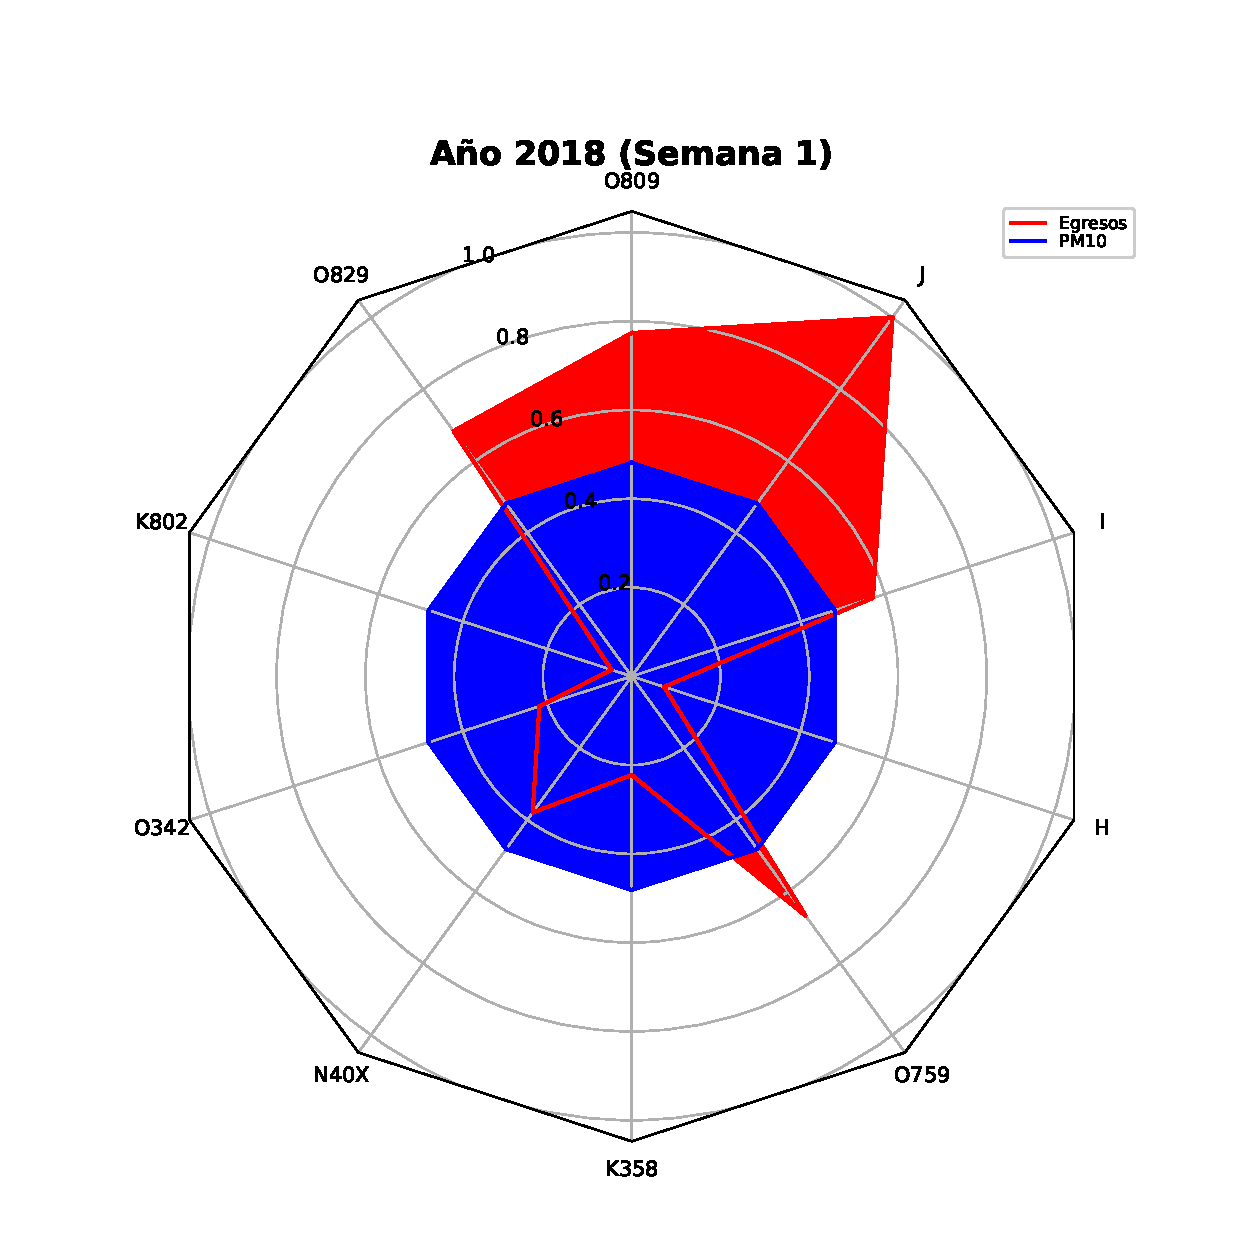
\includegraphics[width=1\textwidth]{spiderweb_PM10_2018_1.eps}
   \end{center}
    \caption[Ejemplo de gráfico de radar]{Nivel del contaminante PM10 y egresos por CIE en la semana 1 del año 2018.}
    \label{grafico_de_telaraña}
\end{figure}

\clearpage
\subsection{Implementación de modelos}
Después de haber generado gráficos para la visualización de la evolución de las variables, se procede a generar modelos para el estudio de la relación entre las variables. Para ello se utiliza \texttt{Python} y la librería \texttt{Statsmodels} \ref{tab:Herramientas utilizadas}. Los tipos de modelos generados se discuten a continuación.

\subsubsection{Regresión lineal}
Primeramente se calcula el coeficiente de correlación de Pearson, si el valor de la correlación se encuentre entre -1 y 1 significa que existe una dependencia lineal y que existe sustento para el modelo de regresión lineal. El modelo de regresión lineal arroja un valor de $R^2$ que indica en que grado la variable independiente explica la varianza de la variable dependiente. Además, se obtiene el valor $p$ que indica la relevancia del resultado y se obtiene la raíz de error cuadrático medio (RMSE) que indica cuantas unidades se alejan los valores predichos por el modelo de los valores reales, eso ayuda a determinar el error del modelo.

\subsubsection{Regresión lineal múltiple}
En los modelos de regresión lineal múltiple se tiene más de una variable independiente. Al obtener el valor de la correlación entre -1 y 1 para verificar que existe sustento para el modelo de regresión lineal, se procede a generar el modelo de regresión lineal múltiple. El modelo de regresión lineal múltiple arroja un valor de $R^2$ que indica en que grado las variables independientes explican la varianza de la variable dependiente. Además, se obtiene el valor $p$ que indica la relevancia del resultado y se obtiene la raíz de error cuadrático medio (RMSE) que indica cuantas unidades se alejan los valores predichos por el modelo de los valores reales, eso ayuda a determinar el error del modelo.

\section{Implementación de la solución propuesta}
% Recapitulando las fases anteriores, se conoce que...
En implementación de la solución propuesta se muestra el desarrollo realizado de los puntos planteados en \ref{Diseño de la solución propuesta}. El desarrollo del presente proyecto se encuentra en el siguiente repositorio Github: \url{https://github.com/selenebpradop/relaciones-contaminantes-salud/}.

\begin{description}
\item{En la función \ref{lst:c1} se muestra el proceso realizado para el procesamiento y agrupamiento de los datos en semanas epidemiológicas.}
\item{El fragmento de código \ref{lst:c2} muestra como es que se generan las series de tiempo, esto después de haber procesado y agrupado los datos.}
\item{La función mostrada en \ref{lst:c3} genera gráficos de radar al ingresarle como parámetros los datos ya procesados y agrupados.}
\item{En el fragmento de código \ref{lst:c4} se muestra como son generados los modelos de regresión lineal después de haber procesado y agrupado los datos.}
\end{description}

\clearpage

\begin{lstlisting}[language=Python, caption=Procesamiento y agrupamiento de datos, label=lst:c1]
import pandas as pd
from epiweeks import Week, date
from sklearn import preprocessing
import seaborn as sns
import matplotlib.pyplot as plt
import string

columns = ['timestamp', contaminante]
dataframec = pd.read_csv('filled.csv', usecols=columns).dropna()
strfdt = '%d-%b-%y %H'
dataframec['timestamp'] = pd.to_datetime(dataframec['timestamp'], errors = 'coerce', format=strfdt)
dataframec = dataframec.dropna()
dataframec = dataframec.reset_index(drop=True)
dataframec['timestamp'] = dataframec['timestamp'].apply(lambda x: x.strftime('%Y-%m-%d %H'))
dataframeca = dataframec.loc[dataframec['timestamp'].str.startswith(año)]
dataframeca = dataframeca.reset_index(drop=True)
strfdt = '%Y-%m-%d %H'
dataframeca['timestamp'] = pd.to_datetime(dataframeca['timestamp'], errors = 'coerce', format=strfdt)
dataframeca['sem'] = dataframeca['timestamp'].apply(lambda x: date(x.year, x.month, x.day))
dataframeca['sem'] = dataframeca['sem'].apply(lambda x: Week.fromdate(x))
dataframeca['sem'] = dataframeca['sem'].apply(lambda x: x.week)
colums = ['EGRESO', 'DIAG_INI']
csvegresos = 'EGRESO_' + año + '.csv'
dataframeea = pd.read_csv(csvegresos, usecols=colums).dropna()
dataframeea['EGRESO'] = pd.to_datetime(dataframeea['EGRESO'], errors = 'coerce', format=strfdto)
dataframeea = dataframeea.loc[dataframeea['ENTIDAD'] == entidad]
dataframeea = dataframeea.dropna()
dataframeea = dataframeea.reset_index(drop=True)
numaño = int(año) 
dataframeea['sem'] = dataframeea['EGRESO'].apply(lambda x: date(x.year, x.month, x.day))
dataframeea['sem'] = dataframeea['sem'].apply(lambda x: Week.fromdate(x))
dataframeea['sem'] = dataframeea['sem'].apply(lambda x: x.week)
dataframeea['EGRESO'] = dataframeea['EGRESO'].apply(lambda x: x if(x.year==numaño) else pd.NaT)   
dataframeea = dataframeea.dropna()
dataframeea = dataframeea.reset_index(drop=True)
dataframesca = pd.DataFrame()
dataframesca['sem'] = semanas.index
dataframesca[contaminante] = ''
n = len(semanas.index)
for i in range (n):
    registrossem = dataframeca.loc[dataframeca['sem'] == i+1]
    promediocas = registrossem[contaminante].mean()
    dataframesca[contaminante][i] = promediocas
\end{lstlisting}

\begin{lstlisting}[language=Python, caption=Generación de series de tiempo, label=lst:c2]
import pandas as pd
from epiweeks import Week, date
from sklearn import preprocessing
import seaborn as sns
import matplotlib.pyplot as plt
import string

diagnosticosaño = dataframeea['DIAG_INI'].value_counts()
diagnosticosaño = diagnosticosaño.sort_values(ascending = False)
ciesaño = dataframeea.groupby(['DIAG_INI', 'sem']).count()

s_scaler = preprocessing.StandardScaler()
ind = []
n = len(semanas.index)
for i in range (n):
    ind.append(i+1)
letras = []
for letra in string.ascii_uppercase:
    letras.append(str(letra))
# Se inicia un contador para controlar la cantidad de graficos a generar
cont = 0
maximo = 10
mindividuales = 7

# Proceso de generación de las figuras
print('\n' + año)
for name in diagnosticosaño.index:
    if cont < maximo:
        dataframegraficoacc = pd.DataFrame()
        dataframegraficoacc[contaminante] = dataframesca[contaminante]
        dataframegraficoacc = dataframegacc.reindex(ind)
        if cont < mindividuales:
            dataframegacc[name] = ciesaño['EGRESO'][name]
            for i in range (n):
                dataframegacc[contaminante][i+1] = dataframesca[contaminante][i]
            col_names = [contaminante, name]    
        else:
            nameg =  letras[cont]
            ciesagrupadas = dataframeea.loc[dataframeea['DIAG_INI'].str.startswith(nameg)]
            ciesagrupadas = ciesagrupadas['sem'].value_counts()
            dataframegacc[nameg] = ciesagrupadas
            for i in range (n):
                dataframegacc[contaminante][i+1] = dataframesca[contaminante][i]
            col_names = [contaminante, nameg]
        df_s = s_scaler.fit_transform(dataframegacc)
        df_s = pd.DataFrame(df_s, columns=col_names)
        fig, ax = plt.subplots(ncols=1, figsize=(20, 8))
        print('\n' + col_names[0] + ' & ' + col_names[1])
        ax.set_title('Contaminante ' + col_names[0] + ' & CIE ' + col_names[1])
        ax.set_xlabel('Semana del año ' + año)
        sns.kdeplot(data=df_s)
        plt.savefig(contaminante + '/' + col_names[0] + '&' + col_names[1] + '_' + año + '.jpg', format='jpg')
        plt.show()
    cont = cont+1
\end{lstlisting}

\begin{lstlisting}[language=Python, caption=Generación de graficos de radar, label=lst:c3]
def create_spiderwebs(datasets, lenlines, numspiders, title, titles, spoke_labels, colors, typeframe):

    # Set the number of lines of each spiderweb
    N = len(datasets)
    theta = radar_factory(N, frame=typeframe)
    # Set the number of columns and rows
    if (numspiders%2==0):
        numrows = 2
        numcols = int(numspiders/2)
    else:
        numrows = 1
        numcols = numspiders
        
    # Draw the shape of the spiderweb
    fig, axs = plt.subplots(figsize=(8, 8), nrows=numrows, ncols=numcols, subplot_kw=dict(projection='radar'))
    fig.subplots_adjust(wspace=0.5, hspace=0.20, top=0.85, bottom=0.05)
    newn = 0.5
    rgrids = []
    for z in range(lenlines*2):
        rgrids.append(newn)
        newn = newn + 0.5

    # Counter of the number of spiders
    i=0

    # Plot each case on separate axes
    for ax, (titlespiderweb) in zip(axs.flat, titles):
        # Put labels in the lines
        ax.set_rgrids(rgrids)        
        ax.set_title(titlespiderweb, weight='bold', size='medium', position=(0.5, 1.1))
        dataspider = []
        # Normalize data
        for y in range(N):
            currentdata = datasets[y]
            number = currentdata[i]
            nmin = min(currentdata);
            nmax = max(currentdata);
            r = nmax - nmin
            x = (number-nmin)/r
            y = lenlines*x
            dataspider.append(y)
        # Draw the new lines in the spiderweb
        ax.plot(theta, dataspider, color=colors[i])
        ax.fill(theta, dataspider, facecolor=colors[i], alpha=0.25)
        # Put the name of each line in the figure
        ax.set_varlabels(spoke_labels)
        # Increment the counter
        i=i+1
    # Show the figure
    plt.show()
\end{lstlisting}

\begin{lstlisting}[language=Python, caption=Generación de los modelos de regresión lineal, label=lst:c4]
datos = pd.DataFrame(dataframegacc, columns=col_names)
# Gráfico
# ==============================================================================
fig, ax = plt.subplots(figsize=(6, 3.84))
datos.plot(
    x    = col_names[0],
    y    = col_names[1],
    c    = 'firebrick',
    kind = "scatter",
    ax   = ax
)
ax.set_title('Contaminante ' + col_names[0] + ' & CIE ' + col_names[1])

# Correlación lineal entre las dos variables
# ==============================================================================
corr_test = pearsonr(x = datos[col_names[0]].fillna(0), y =  datos[col_names[1]].fillna(0))
print("Coeficiente de correlación de Pearson: ", corr_test[0])
print("P-value: ", corr_test[1])

# División de los datos en train y test
# ==============================================================================
xx = datos[[col_names[0]]].fillna(0)
yy = datos[[col_names[1]]].fillna(0)
        
x2 = xx.values.tolist()
y2 = yy.values.tolist()

# Creación del modelo utilizando matrices como en scikitlearn
# ==============================================================================
# A la matriz de predictores se le tiene que añadir una columna de 1s para el intercept del modelo
x = np.array(x2).astype(float)
y = np.array(y2).astype(float)
#ones = np.ones(len(x[0]))
#X = sm.add_constant(np.column_stack((x[0], ones)))
#for ele in x[1:]:
#    X = sm.add_constant(np.column_stack((ele, X)))
modelo = sm.OLS(y, x)
modelo = modelo.fit()
print(modelo.summary())
\end{lstlisting}
